\documentclass[sigplan,10pt]{acmart}

\settopmatter{printacmref=true,printfolios=true}
\setcopyright{none}
\renewcommand\footnotetextcopyrightpermission[1]{}

\usepackage{xspace}
\usepackage{array}
\usepackage{listings}
\usepackage{xcolor}
\usepackage{subcaption}
\usepackage{tikz}
\usetikzlibrary{arrows.meta,calc}

\lstdefinestyle{asm}{
  basicstyle=\ttfamily\scriptsize,
  columns=fullflexible,
  keepspaces=true,
  commentstyle=\color{gray},
  morecomment=[l]{;},
  morecomment=[l]{//},
}

\usepackage[most]{tcolorbox}


%%
%% \BibTeX command to typeset BibTeX logo in the docs
\AtBeginDocument{%
  \providecommand\BibTeX{{%
    Bib\TeX}}}

%% Rights management information.  This information is sent to you
%% when you complete the rights form.  These commands have SAMPLE
%% values in them; it is your responsibility as an author to replace
%% the commands and values with those provided to you when you
%% complete the rights form.
\setcopyright{acmlicensed}
\copyrightyear{2026}
\acmYear{2026}
\acmDOI{XXXXXXX.XXXXXXX}
%% These commands are for a PROCEEDINGS abstract or paper.
\acmConference[ATC '26]{2026 ACM SIGOPS Annual Technical Conference}{November 16--18,
  2026}{Shatin, Hong Kong}
%%
%%  Uncomment \acmBooktitle if the title of the proceedings is different
%%  from ``Proceedings of ...''!
%%
%%\acmBooktitle{ATC '26: 2026 ACM SIGOPS Annual Technical Conference,
%%  November 16--18, 2026, Shatin, Hong Kong}
\acmISBN{978-1-4503-XXXX-X/2026/11}


%%
%% Submission ID.
%% Use this when submitting an article to a sponsored event. You'll
%% receive a unique submission ID from the organizers
%% of the event, and this ID should be used as the parameter to this command.
%%\acmSubmissionID{123-A56-BU3}

%%
%% For managing citations, it is recommended to use bibliography
%% files in BibTeX format.
%%
%% You can then either use BibTeX with the ACM-Reference-Format style,
%% or BibLaTeX with the acmnumeric or acmauthoryear sytles, that include
%% support for advanced citation of software artefact from the
%% biblatex-software package, also separately available on CTAN.
%%
%% Look at the sample-*-biblatex.tex files for templates showcasing
%% the biblatex styles.
%%

%%
%% The majority of ACM publications use numbered citations and
%% references.  The command \citestyle{authoryear} switches to the
%% "author year" style.
%%
%% If you are preparing content for an event
%% sponsored by ACM SIGGRAPH, you must use the "author year" style of
%% citations and references.
%% Uncommenting
%% the next command will enable that style.
%%\citestyle{acmauthoryear}


%%
%% end of the preamble, start of the body of the document source.
\begin{document}

%%
%% The "title" command has an optional parameter,
%% allowing the author to define a "short title" to be used in page headers.
\title{\tool: Safely Optimizing eBPF through Instruction Extensions}

\author{Yusheng Zheng$^{1*}$, Zhengjie Ji$^{2*}$, Weichen Tao$^{3}$, Hao Sun$^{4}$, Wei Zhang$^{5}$, Dan Williams$^{2}$, Andi Quinn$^{1}$}
\thanks{$^*$Equal contribution.}
\affiliation{%
  \institution{$^{1}$UC Santa Cruz \quad $^{2}$Virginia Tech \quad $^{3}$Telecom Paris \quad $^{4}$ETH Zurich \quad $^{5}$University of Connecticut}
  \country{}}
\renewcommand{\authorsaddresses}{}

%%
%% By default, the full list of authors will be used in the page
%% headers. Often, this list is too long, and will overlap
%% other information printed in the page headers. This command allows
%% the author to define a more concise list
%% of authors' names for this purpose.
\renewcommand{\shortauthors}{Zheng et al.}

%%
%% The abstract is a short summary of the work to be presented in the
%% article.
\newcommand{\zj} [1]{\textcolor{blue}{{}#1}}
\newcommand{\note} [1]{\textcolor{red}{#1}}

\newcommand{\tool}{\textsc{BPF-Ext}\xspace}
\newcommand{\kinsn}{\textsc{Kinsn}\xspace}
\newcommand{\kinsns}{\textsc{Kinsn}s\xspace}
\newcommand{\lang}{\kinsn}

\newcommand{\citehere}[1][?]{  \textcolor{red}{[#1]}}

\newtcolorbox[auto counter]{finding}[1][]{
  enhanced, breakable, sharp corners,
  fontupper=\normalfont\normalsize,
  colback=black!4, colframe=black!75, boxrule=0.5pt,
  left=2.2mm, right=2.2mm, top=1.4mm, bottom=1.4mm,
  before skip=2.4mm, after skip=2.4mm,
  #1,
}
\newcommand{\finlabel}{\textbf{Finding~\thetcbcounter:}\ }

\begin{abstract}
eBPF lets applications execute custom logic in the kernel for tasks such as packet processing and system observability. However, the existing compilation pipeline fails to select efficient implementations available on the target CPU for some computations. Exploiting these opportunities requires existing approaches to trade off native optimization capability against the complexity of trusted code. Bytecode rewriting is constrained by the existing JIT's instruction-selection rules, whereas adding native optimizations requires trusting the corresponding program transformations and code generation. We present \tool, an extensible eBPF compilation framework that enables more efficient native implementations while reusing the existing verifier for safety analysis. The framework identifies optimization opportunities in userspace and selects native implementations provided by the kernel through extended instructions. Each extension describes its behavior using eBPF instructions for safety analysis within the complete program and executes using a semantically equivalent native implementation. We implement seven categories of local optimizations on x86-64 and ARM64. Relative to the stock Linux eBPF JIT, microbenchmarks achieve geometric mean speedups of 1.24$\times$ and 1.22$\times$, respectively. Throughput increases by 7.4\% for Cilium on x86-64 and by 7.3\% for Katran on ARM64.
\end{abstract}


%%
%% The code below is generated by the tool at http://dl.acm.org/ccs.cfm.
%% Please copy and paste the code instead of the example below.
%%
\begin{CCSXML}
<ccs2012>
 <concept>
  <concept_id>10011007.10011006.10011008.10011009.10011015</concept_id>
  <concept_desc>Software and its engineering~Just-in-time compilers</concept_desc>
  <concept_significance>500</concept_significance>
 </concept>
 <concept>
  <concept_id>10011007.10011006.10011039</concept_id>
  <concept_desc>Software and its engineering~Formal language definitions</concept_desc>
  <concept_significance>300</concept_significance>
 </concept>
 <concept>
  <concept_id>10010520.10010553.10010562</concept_id>
  <concept_desc>Computer systems organization~Embedded systems</concept_desc>
  <concept_significance>300</concept_significance>
 </concept>
 <concept>
  <concept_id>10011007.10011006.10011041</concept_id>
  <concept_desc>Software and its engineering~Compilers</concept_desc>
  <concept_significance>300</concept_significance>
 </concept>
</ccs2012>
\end{CCSXML}

\ccsdesc[500]{Software and its engineering~Just-in-time compilers}
\ccsdesc[300]{Software and its engineering~Formal language definitions}
\ccsdesc[300]{Computer systems organization~Embedded systems}
\ccsdesc[300]{Software and its engineering~Compilers}

%%
%% Keywords. The author(s) should pick words that accurately describe
%% the work being presented. Separate the keywords with commas.
\keywords{eBPF, JIT compilation, kernel extensions, instruction set extension, verified compilation, proof-carrying code}

% \received{20 February 2007}
% \received[revised]{12 March 2009}
% \received[accepted]{5 June 2009}

%%
%% This command processes the author and affiliation and title
%% information and builds the first part of the formatted document.
\maketitle
\fancyhf{}
\fancyfoot[C]{\thepage}
\renewcommand{\headrulewidth}{0pt}

\section{Introduction}
\label{sec:introduction}

eBPF is a technology for safely extending operating system kernels. It lets applications execute custom logic in the kernel for tasks such as packet processing~\cite{katran} and system observability~\cite{bpftrace}. Execution efficiency is an important requirement for these extensions. For example, on a network path that processes each packet, the eBPF program runs for every packet, so its execution cost affects CPU overhead and packet-processing capacity.

However, the existing eBPF compilation pipeline fails to select efficient implementations available on the target CPU for some computations. A userspace compiler first produces eBPF bytecode. After the kernel verifier~\cite{verifier} checks it, the in-kernel eBPF just-in-time (JIT) compiler generates native code. Some computations are decomposed into multiple basic operations in the bytecode. The current JIT mainly translates instructions individually and does not recombine these sequences into corresponding native operations. For example, a 64-bit rotation by a constant is represented as shifts and bitwise OR in the bytecode. The existing x86-64 JIT translates these operations separately, producing multiple native instructions. Direct native compilation can instead perform the same computation with a single rotate instruction.

Existing optimization approaches face different limitations in using these native implementations. Userspace optimizers such as K2~\cite{xu2021synthesizing} improve programs by rewriting existing eBPF instructions, but the resulting bytecode still goes through the existing JIT. Bytecode rewriting alone therefore cannot add native instruction-selection rules that the JIT lacks. Extending the JIT directly can add these rules, but requires maintaining and reviewing the corresponding pattern recognition, transformations, and code generation in the kernel. These transformations run after verification, so errors can also invalidate the verified safety conditions. Shahinfar et al.~\cite{shahinfar2026fun} propose native optimization in userspace after verification. This moves optimization code out of the kernel but requires trusting the userspace optimizer's translation.

To avoid adding a complex optimizer to the trusted code, we separate optimization selection from safety checking. The same local computation can have an eBPF implementation and a native implementation. The former is used for safety analysis of the complete program, and the latter for execution. Both must exhibit the same program-observable behavior for the safety analysis to apply to the code that executes.

We present \tool, an extensible framework for eBPF compilation that enables more efficient native implementations while reusing the existing verifier for safety analysis. A userspace pattern recognizer specifies operations and their parameters using extended instructions called \kinsns. The kernel checks their usage conditions and expands them into existing eBPF instructions, which the verifier analyzes with the rest of the program. After verification succeeds, the JIT generates code using semantically equivalent native implementations. We organize equivalence proofs around a shared operation specification and demonstrate a rotation proof in Lean~4~\cite{moura2021lean}. New recognition rules can reuse existing \kinsns. New operations reuse the framework's mechanisms for verification and code generation.

We implement \tool in Linux for x86-64 and ARM64, using kernel modules to provide seven categories of local optimizations involving computation, control flow, and memory access. With the stock Linux eBPF JIT as the baseline, the geometric mean microbenchmark speedups on the two architectures are 1.24$\times$ and 1.22$\times$, respectively. Throughput increases by 7.4\% for Cilium on x86-64 and by 7.3\% for Katran on ARM64. These results show that the framework's local optimizations improve the execution efficiency of computational microbenchmarks and the packet processing throughput of real applications.

\noindent\textbf{Contributions.}
We make the following contributions:
\begin{itemize}
    \item We investigate performance differences between eBPF and direct native compilation, and use code comparisons to identify local optimization opportunities that the existing pipeline leaves unused.
    \item We present \tool, connecting userspace pattern recognition to in-kernel native implementations via extended instructions, and methods to reuse existing safety analysis and prove semantic equivalence.
    \item We implement the framework and seven categories of local optimizations on x86-64 and ARM64, and evaluate their performance and overhead using microbenchmarks and packet-processing applications.
\end{itemize}
\section{The eBPF Compilation Pipeline}
\label{sec:background}

The eBPF compilation pipeline translates source programs into code for execution in the kernel and checks program safety before execution, as shown in Figure~\ref{fig:ebpf}. A user-space compiler first produces eBPF bytecode, which the kernel verifies at load time. When just-in-time (JIT) compilation is used, the eBPF JIT then generates machine code for the target architecture. Once loaded, the program can be attached to a kernel hook, such as XDP or a tracepoint, and executed in response to the corresponding events~\cite{linuxndlibbpf}.

\begin{figure}[t]
  \centering
  \fontencoding{T1}\selectfont
  \renewcommand{\sfdefault}{lmss}
  \renewcommand{\ttdefault}{lmtt}
\definecolor{ink}{gray}{0}
\definecolor{compilefill}{HTML}{EEE7F2}
\definecolor{kernelfill}{HTML}{E5EDF8}
\definecolor{hookfill}{HTML}{FFF0CA}

\newcommand{\programartifact}[3]{\coordinate (#1) at (#2,#3);
  \coordinate (#1-south) at ($(#1)+(0,-0.35)$);
  \draw[draw=ink,fill=white,line width=0.55pt]
    ($(#1)+(-0.25,-0.35)$) -- ($(#1)+(0.25,-0.35)$)
    -- ($(#1)+(0.25,0.18)$) -- ($(#1)+(0.08,0.35)$)
    -- ($(#1)+(-0.25,0.35)$) -- cycle;
  \draw[draw=ink,line width=0.55pt]
    ($(#1)+(0.08,0.35)$) -- ($(#1)+(0.08,0.18)$)
    -- ($(#1)+(0.25,0.18)$);
  \node[font=\ttfamily\bfseries\fontsize{6.5}{6.5}\selectfont,
    text=ink,inner sep=0pt] at ($(#1)+(0,-0.06)$) {</>};
}

\resizebox{\linewidth}{!}{\begin{tikzpicture}[
  x=1cm,y=1cm,
  font=\sffamily\fontsize{8.5}{10}\selectfont,
  text=ink,
  component/.style={rectangle,draw=ink,line width=0.55pt,
    minimum width=1.50cm,minimum height=1.00cm,
    text width=1.18cm,inner xsep=1.6mm,inner ysep=1.5mm,
    outer sep=0pt,align=center},
  artifactlabel/.style={align=center,inner sep=0pt,outer sep=0pt,
    font=\sffamily\fontsize{8}{9}\selectfont,fill=white},
  flow/.style={-{Stealth[length=1.4mm,width=1.0mm]},
    draw=ink,line width=0.6pt},
  edgeword/.style={font=\sffamily\fontsize{8}{9}\selectfont,
    inner sep=0pt,outer sep=0pt,fill=white}
]
  \path[use as bounding box] (0,0) rectangle (8.5,4.95);

  \node[anchor=base west,font=\sffamily\bfseries\fontsize{8.5}{10}\selectfont]
    at (0.03,4.63) {User space};
  \node[anchor=base west,font=\sffamily\bfseries\fontsize{8.5}{10}\selectfont]
    at (2.12,4.63) {Kernel};
  \draw[draw=ink,line width=0.55pt,dash pattern=on 2pt off 2pt]
    (1.95,1.40) -- (1.95,4.89);

  \node[component,fill=compilefill] (compiler) at (0.80,2.00)
    {Clang};
  \node[component,fill=kernelfill] (verifier) at (3.10,2.00)
    {eBPF\\verifier};
  \node[component,fill=kernelfill] (jit) at (5.40,2.00)
    {eBPF\\JIT};
  \node[component,rounded corners=5mm,fill=hookfill] (hook) at (7.70,2.00)
    {Hook\\point};

  \programartifact{source}{0.80}{3.55}
  \node[artifactlabel,anchor=south] at (0.80,4.10) {Source code};
  \node[artifactlabel,anchor=south] at (7.70,3.40) {Event};

  \draw[flow] (source-south) -- (compiler.north);
  \draw[flow] (7.70,3.20) --
    node[edgeword,left=2mm] {Trigger} (hook.north);

  \draw[flow] (compiler.east) -- (verifier.west);
  \draw[flow] (verifier.east) -- (jit.west);
  \draw[flow] (jit.east) -- (hook.west);

  \programartifact{bytecode}{1.95}{0.85}
  \programartifact{verified}{4.25}{0.85}
  \programartifact{native}{6.55}{0.85}
  \node[artifactlabel,anchor=north] at (1.95,0.30) {eBPF bytecode};
  \node[artifactlabel,anchor=north] at (4.25,0.30) {Verified bytecode};
  \node[artifactlabel,anchor=north] at (6.55,0.30) {Native code};
\end{tikzpicture}}
  \caption{The eBPF compilation and execution pipeline. Bytecode is verified and compiled into native code at load time. Once the program is attached to a hook, the corresponding events trigger its execution.}
  \Description{A user-space Clang compiler produces eBPF bytecode. In the kernel, the eBPF verifier checks the bytecode and the eBPF JIT compiles it to native code. After the program is attached to a hook, events trigger its execution.}
  \label{fig:ebpf}
\end{figure}


\noindent\textbf{Source compilation.}
Clang optimizes source programs in user space and compiles them into eBPF bytecode. Its front end first translates C source into LLVM intermediate representation (IR), which LLVM optimizes before the eBPF back end performs instruction selection and register allocation~\cite{llvmndcodegenerator}. This stage targets the eBPF instruction set; the JIT then generates machine code for the target CPU.

\noindent\textbf{Verification.}
The kernel checks an eBPF program's safety through static analysis at load time. The verifier analyzes changes to register and stack states along the program's control flow. For example, it uses a pointer's offset range and the access size to determine whether a memory access could exceed the bounds of the referenced region~\cite{verifier}. The loading process also performs necessary bytecode transformations before passing the accepted program to the JIT compiler.

\noindent\textbf{JIT compilation.}
The eBPF JIT translates bytecode into machine code for the target architecture. The x86-64 and ARM64 implementations map eBPF registers to fixed native registers and select native instructions and encodings based on the target architecture and instruction operands~\cite{linux_bpf_jit,linuxndarm64jit}. For example, on x86-64, a register can be set to zero either by a \texttt{MOV} instruction that writes an immediate zero or by an \texttt{XOR} instruction with the same register as both operands, since the bitwise exclusive OR of a value with itself is zero. The eBPF JIT selects the latter for its shorter encoding~\cite{linux_bpf_jit}. Despite these local optimizations, programs compiled through the eBPF pipeline can still run more slowly than programs compiled directly to native code from the same source. Section~\ref{sec:characterization} quantifies this difference and investigates its sources.
\section{Investigating eBPF Performance Bottlenecks}
\label{sec:characterization}

A program compiled through the eBPF pipeline can run more slowly than native code compiled directly from the same source. This section quantifies the difference, investigates its sources, and discusses approaches to improving performance and the requirements they must meet.

\noindent\textbf{Microbenchmarks.}
We use 27 computational microbenchmarks to examine how compilation paths affect execution time. The benchmarks include simplified application logic and programs constructed around specific computations. For example, the Katran~\cite{katran} benchmark retains packet hashing and destination selection. Table~\ref{tab:microbenchmarks} lists their main computations. Their computation bodies make no helper calls or map accesses, reducing the influence of kernel services. All paths use the same computation source and fixed inputs.

\begin{table*}[t]
\centering
\small
\caption{Computational microbenchmarks used in Figure~\ref{fig:char-pure-percase}. The \texttt{cksum} and \texttt{tc\_cksum} programs perform the same computation with different eBPF program types.}
\label{tab:microbenchmarks}
\renewcommand{\arraystretch}{1.08}
\begin{tabular*}{\textwidth}{@{\extracolsep{\fill}}ll@{\hspace{1.2em}}ll@{\hspace{1.2em}}ll@{}}
\toprule
\textbf{Benchmark} & \textbf{Computation} & \textbf{Benchmark} & \textbf{Computation} & \textbf{Benchmark} & \textbf{Computation} \\
\midrule
\texttt{bitmap} & Bit counting, mixing & \texttt{katran} & Hash-based selection & \texttt{sock\_lb} & Service selection \\
\texttt{rule\_scan} & First-match scan & \texttt{policy} & Nested conditions & \texttt{tcpconn} & Connection filtering \\
\texttt{runqlat} & Logarithmic buckets & \texttt{siphash} & SipHash-style mixing & \texttt{tetragon} & Process-event filtering \\
\texttt{trace\_sw} & Switch dispatch & \texttt{bounds} & Bounds checks, reads & \texttt{otel} & Frame-record scan \\
\texttt{cksum} & Checksum & \texttt{field} & Field reads, mixing & \texttt{ct\_nat} & Address rewriting \\
\texttt{memcmp} & Bytewise comparison & \texttt{bitfield} & Bit-field extraction & \texttt{toeplitz} & Toeplitz-style hashing \\
\texttt{vlan} & Packet-header parsing & \texttt{str\_search} & Substring search & \texttt{fnv} & FNV-1a hashing \\
\texttt{call\_fanout} & Local-call dispatch & \texttt{syscall\_lookup} & Syscall label lookup & \texttt{tc\_cksum} & Checksum (TC) \\
\texttt{5tuple} & Jenkins-style hashing & \texttt{http} & HTTP prefix detection & \texttt{cgroup} & Hash mixing \\
\bottomrule
\end{tabular*}
\end{table*}


\noindent\textbf{Experimental setup.}
We use EC2 c7i.large instances for x86-64 and c7g.large instances for ARM64. The experiments use Clang 18.1.3 and a research kernel based on Linux 7.0.0-rc2. For each path, we take repeated measurements after warmup on 12 independent instances and compare mean execution time per invocation, excluding loading and compilation.

\subsection{Quantifying eBPF Slowdown}
\label{subsec:char-slowdown}

We compare execution time between the eBPF JIT and user-space native paths, using the same source and \texttt{-O2} for both. The eBPF path produces bytecode, which the kernel verifies and JIT-compiles before repeated execution through \texttt{BPF\_PROG\_TEST\_RUN}. The user-space native path compiles directly to native code and repeatedly invokes it through a function pointer.

\begin{figure*}[t]
\centering
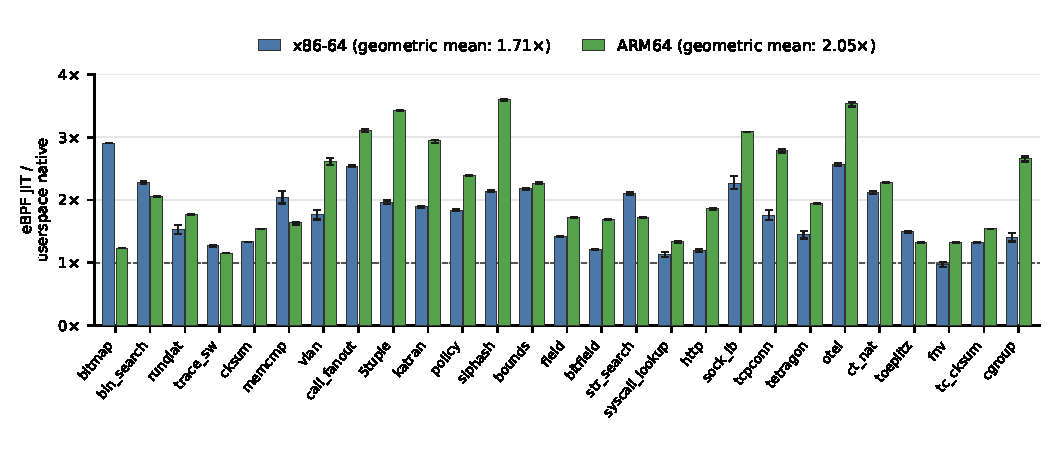
\includegraphics[width=\textwidth]{figures/sec-3-slowdown-o2-grouped.pdf}
\caption{eBPF JIT execution time relative to user-space native. The left and right bars for each benchmark correspond to x86-64 and ARM64. Each bar is the ratio of mean per-call execution times on the same architecture; values above 1 indicate slower eBPF JIT execution, and the dashed line denotes equal time. Error bars show 95\% confidence intervals obtained by resampling instances. Each geometric mean in the legend summarizes the 27 benchmark ratios for that architecture.}
\Description{Grouped bars compare eBPF JIT with user-space native across 27 benchmarks. Blue bars represent x86-64 and green bars represent ARM64, with geometric mean execution-time ratios of 1.71 and 2.05, respectively.}
\label{fig:char-pure-percase}
\end{figure*}


Figure~\ref{fig:char-pure-percase} shows that, across these benchmarks, programs generally run more slowly through the eBPF path than when compiled directly to native code from the same source. The geometric mean execution-time ratios are 1.71 on x86-64 and 2.05 on ARM64. For FNV on x86-64, the two paths have similar execution times. Machine-code comparisons show that both retain the byte-by-byte hash recurrence of exclusive OR and multiplication; direct native compilation does not shorten this dependency chain.

\subsection{Investigating Sources of eBPF Slowdown}
\label{subsec:char-sources}
\label{subsec:char-idiom}

To investigate why eBPF programs run more slowly than user-space native programs compiled from the same source, we first examine whether the difference in execution location explains the slowdown. We run the user-space native compilation output in the kernel through the same test-run interface as the eBPF JIT. Both native paths use only general-purpose registers, so kernel execution requires no additional saving and restoring of floating-point or SIMD registers~\cite{linuxndfloatingpoint}.

Table~\ref{tab:char-micro-summary} shows that the performance advantage of direct native compilation persists in the kernel. Although kernel native execution takes about 6\% longer than user-space native execution on x86-64 and 15\% longer on ARM64 overall, it remains faster than JIT-compiled eBPF code running in the same kernel.

\begin{finding}[unbreakable]
\finlabel Execution location does not fully explain the performance difference between the eBPF JIT and direct native compilation. With both running in the kernel, JIT-compiled eBPF code still takes 1.62$\times$ as long as native code on x86-64 and 1.77$\times$ on ARM64 overall.
\end{finding}

We next examine whether limitations of eBPF bytecode itself account for the performance difference between the eBPF JIT and direct native compilation. We compare native code regenerated from eBPF bytecode with directly compiled native code, running both in user space. LLVM-BPF~\cite{zheng2025extending} is an LLVM-based user-space eBPF compiler that translates bytecode into LLVM IR, optimizes it, and generates native code. We give LLVM-BPF the same bytecode as the eBPF JIT, use O2 optimization, and select the same target CPU and instruction features as direct native compilation. Table~\ref{tab:char-micro-summary} shows that LLVM-BPF approaches the overall performance of direct native compilation, demonstrating that these programs can still have efficient implementations after passing through eBPF bytecode.

\begin{table}[t]
\centering
\small
\caption{Execution-time ratios on x86-64 and ARM64. Each entry is the geometric mean of the 27 ratios of mean per-call execution times, with the numerator and denominator given in the first column. Values above 1 indicate a slower numerator path.}
\label{tab:char-micro-summary}
\begin{tabular}{@{}lcc@{}}
\toprule
\textbf{Execution-time ratio} & \textbf{x86-64} & \textbf{ARM64} \\
\midrule
Kernel native / user-space native & 1.055 & 1.154 \\
\addlinespace
eBPF JIT / kernel native & 1.622 & 1.773 \\
\addlinespace
LLVM-BPF / user-space native & 1.068 & 1.054 \\
\bottomrule
\end{tabular}
\end{table}


\begin{finding}[unbreakable]
\finlabel Using eBPF bytecode does not prevent these programs from approaching the overall performance of direct native compilation. In user space, code generated by LLVM-BPF takes about 7\% longer than native code on x86-64 and 5\% longer on ARM64 overall.
\end{finding}

We further analyze why the eBPF compilation pipeline does not fully exploit the target CPU's instructions. LLVM's BPF back end optimizes and selects instructions for the eBPF instruction set, whereas direct native compilation targets the final CPU~\cite{llvmndcodegenerator}. Some computations that a single native instruction can perform therefore require multiple basic operations in bytecode. eBPF is designed to make it easy for a JIT to map basic instructions to native architectures~\cite{linuxndclassicbpf}. Selecting a native instruction for the full computation requires recognizing how its basic operations relate.

The rotation in Figure~\ref{fig:jit-dump} illustrates this process. eBPF has no rotate instruction~\cite{rfc9669}, so LLVM's BPF back end expands rotations into basic operations~\cite{llvmndbpflowering}. A 64-bit left rotation by 16 bits in the SipHash-style microbenchmark consists of a copy, two shifts, and a bitwise OR. The current x86-64 JIT emits \texttt{MOV; SHR; SHL; OR}, whereas direct native compilation emits a single \texttt{RORX}. The bytecode fully preserves the rotation computation, but expresses it across several instructions. The current JIT selects native implementations from each instruction's opcode and operands, retaining this sequence because it does not analyze their data dependencies to recognize rotation.

\begin{figure}[t]
\centering
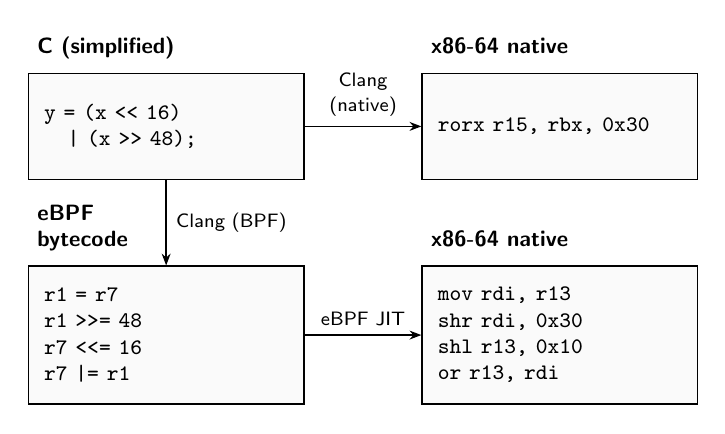
\begin{tikzpicture}[
  x=1cm,y=1cm,
  font=\sffamily\fontsize{8}{9.5}\selectfont,
  code/.style={draw=black,line width=0.5pt,fill=black!2,
    text width=3.1cm,inner xsep=2mm,inner ysep=2mm,
    anchor=north west,align=left,
    font=\ttfamily\fontsize{8}{9.5}\selectfont},
  heading/.style={anchor=south west,text depth=1.5pt,font=\sffamily\bfseries\fontsize{8}{9.5}\selectfont},
  flow/.style={-{Stealth[length=1.5mm]},line width=0.6pt},
  stage/.style={align=center,font=\sffamily\fontsize{7.5}{9}\selectfont}
]
\path[use as bounding box] (0,-0.08) rectangle (8.5,4.72);
\node[heading] at (0,4.21) {C (simplified)};
\node[heading] at (5,4.21) {x86-64 native};
\node[code,minimum height=1.35cm] (source) at (0,4.15) {y = (x <{}< 16)\\\hspace*{1em}| (x >{}> 48);};
\node[code,minimum height=1.35cm] (native) at (5,4.15) {rorx r15, rbx, 0x30};
\node[heading,align=left] at (0,1.76) {eBPF\\bytecode};
\node[heading] at (5,1.76) {x86-64 native};
\node[code,minimum height=1.75cm] (bytecode) at (0,1.70) {r1 = r7\\r1 >{}>= 48\\r7 <{}<= 16\\r7 |= r1};
\node[code,minimum height=1.75cm] (jit) at (5,1.70) {mov rdi, r13\\shr rdi, 0x30\\shl r13, 0x10\\or r13, rdi};
\draw[flow] (source.east) -- node[above,stage] {Clang\\(native)} (native.west);
\draw[flow] (source.south) -- node[right,stage] {Clang (BPF)} (bytecode.north);
\draw[flow] (bytecode.east) -- node[above,stage] {eBPF JIT} (jit.west);
\end{tikzpicture}
\caption{Two compilation paths for a 64-bit left rotation by 16 bits in the SipHash-style benchmark on x86-64. In the simplified C expression, \texttt{x} and \texttt{y} are 64-bit unsigned integers. The code panels show only the rotation, omitting input preparation and adjacent computation. Assembly uses Intel syntax; right rotation by \texttt{0x30} (48) bits equals left rotation by 16 bits.}
\Description{A two-by-two diagram compares direct native compilation with compilation through eBPF. Simplified C for the constant-16 rotation produces one RORX instruction through direct compilation, or a register copy, two shifts, and an OR through eBPF and its JIT.}
\label{fig:jit-dump}
\end{figure}


Table~\ref{tab:isa-gap} compares the generated code for bit extraction and big-endian reads, which also offer opportunities to combine basic operations or memory accesses. The halfword load and byte-order conversion needed for the big-endian read already exist in the eBPF instruction set. These opportunities extend beyond computations without a dedicated eBPF instruction.

\begin{table*}[t]
\centering
\small
\caption{Native instruction sequences for two computations in the compiled programs. The operand \texttt{b} is a zero-extended byte. Bit extraction starts with the operand ready; the big-endian read includes the memory loads.}
\label{tab:isa-gap}
\begin{tabular}{@{}llll@{}}
\toprule
\textbf{Computation} & \textbf{Architecture} & \textbf{eBPF JIT} & \textbf{Direct native} \\
\midrule
\texttt{(b >{}> 1) \& 0x1f} & ARM64 & \texttt{LSR; AND} & \texttt{UBFX} \\
Big-endian 16-bit read & x86-64 & \texttt{MOVZX} $\times$ 2\texttt{; SHL; OR; AND} & \texttt{MOVBE; MOVZX} \\
Big-endian 16-bit read & ARM64 & \texttt{LDRB} $\times$ 2\texttt{; LSL; ORR; AND} & \texttt{LDRH; REV16} \\
\bottomrule
\end{tabular}
\end{table*}


\begin{finding}[unbreakable]
\finlabel The current eBPF compilation pipeline misses some opportunities to combine operations for the target CPU. User-space compilation produces combinations of basic eBPF operations, while the subsequent JIT mainly maps individual instructions without recognizing the combinations that enable more compact native code.
\end{finding}

\subsection{Design Implications}
\label{subsec:char-challenges}

The code comparisons show that some combinations of operations admit more compact native implementations. Taking advantage of these opportunities requires recognizing these combinations in a program and selecting their implementations for the target architecture.

Existing approaches have limitations in supporting these native optimizations. K2~\cite{xu2021synthesizing}, Merlin~\cite{mao2024merlin}, and EPSO~\cite{zhu2025epso} rewrite programs in user space, combining operations and eliminating redundancy using existing eBPF instructions, then pass the results to the existing verifier and JIT. These methods can improve generated code, but rewriting ordinary bytecode alone cannot select a native implementation for which the JIT has no selection rule. Enhancing the JIT directly can add such rules, but requires adding the corresponding pattern analysis, transformation checks, and code generation to the kernel. As the set of optimizations grows, so does the kernel code that must be maintained and reviewed. In addition, these transformations occur after verification: incorrect matching or code generation can change program behavior and invalidate the safety guarantee established by the verifier. Shahinfar et al.~\cite{shahinfar2026fun} propose generating native code directly with a user-space optimizer after verification. This keeps the optimization implementation outside the kernel, but safe execution still requires a trusted translation process or additional checks on the generated code.

We investigate how to integrate local native operations while limiting the size and complexity of the trusted code added to the kernel. Extensions must preserve observable program behavior across optimization and ensure that the verifier's safety conclusions apply to the machine code that executes. New operations should then reuse the integration and verification mechanisms and support native implementations of the same operation across architectures, reducing extension and maintenance costs. Section~\ref{sec:mechanism} describes the design of \tool.

\section{\tool Design}
\label{sec:mechanism}

This section describes how \tool uses more efficient native implementations for eBPF programs while preserving their safety guarantees. We introduce extended instructions and their optimization mechanism (\S\ref{subsec:pipeline}), explain the additional kernel safety responsibilities and trusted code (\S\ref{subsec:safety}), and describe how to prove that the verification and execution implementations have the same semantics (\S\ref{sec:formal-verification}).

\subsection{Optimizing eBPF Programs with \kinsns}
\label{subsec:pipeline}

\tool places pattern recognition in userspace and provides the corresponding native implementations in the kernel. The userspace pattern recognizer rewrites matched code as extended instructions that specify operations and their parameters while preserving program behavior. We call these extended instructions \kinsns. The kernel generates code for the operation specified by each \kinsn, so the JIT need not rediscover the original code pattern.

\begin{figure*}[t]
\centering
\begingroup
\fontencoding{T1}\selectfont
\renewcommand{\sfdefault}{lmss}
\renewcommand{\ttdefault}{lmtt}
\definecolor{evoink}{HTML}{17365D}
\definecolor{evogreen}{HTML}{EDF2F8}
\definecolor{evoedge}{HTML}{506C8B}
\definecolor{evoblue}{HTML}{E5EDF8}
\definecolor{evopurple}{HTML}{EEE7F2}
\definecolor{evobaseline}{HTML}{B56A00}
\begin{tikzpicture}[
x=1cm,y=1cm,font=\sffamily\fontsize{8.5}{10}\selectfont,
code/.style={anchor=west,font=\ttfamily\fontsize{8}{10}\selectfont,inner sep=0pt},
slot/.style={anchor=west,font=\sffamily\fontsize{7.5}{9}\selectfont,inner sep=0pt,text=evoink},
component/.style={draw,line width=.55pt,fill=evoblue,minimum width=2.20cm,minimum height=1.20cm,text width=1.94cm,align=center,inner xsep=1.3mm,inner ysep=.8mm,outer sep=0pt},
stepdot/.style={circle,fill=evoink,draw=evoink,minimum size=2.2mm,inner sep=0pt,outer sep=0pt},
flow/.style={-{Stealth[length=1.4mm,width=1mm]},line width=.75pt,shorten <=.45mm,shorten >=.45mm},
originalflow/.style={flow,draw=evobaseline,dash pattern=on 5pt off 3pt},
extendedflow/.style={flow,draw=evoink,line width=.85pt},
callarrow/.style={flow,draw=evoink,line width=.55pt,line cap=round,dash pattern=on .5pt off 2.2pt},
resultarrow/.style={flow,draw=evoink,line width=.55pt},
edgelabel/.style={font=\sffamily\fontsize{8}{9}\selectfont,text=evoink,align=center,inner sep=0pt},
regionlabel/.style={font=\sffamily\bfseries\fontsize{8.5}{10}\selectfont,inner sep=0pt},
productnumber/.style={circle,draw=black!75,fill=white,line width=.5pt,minimum size=3.5mm,inner sep=0pt,outer sep=0pt,font=\sffamily\fontsize{7.5}{8}\selectfont},
panelheading/.style={anchor=west,align=left,inner sep=0pt,font=\sffamily\fontsize{8}{10}\selectfont}
]
\path[use as bounding box] (0,0) rectangle (17.5,10.90);
\draw[draw=evoedge,fill=evogreen,line width=.55pt] (3.10,5.15) rectangle (12.30,8.30);
\node[regionlabel] at (7.70,5.475) {BPF-Ext};
\draw[draw=evoedge,fill=white,line width=.5pt] (6.45,5.80) rectangle (11.95,7.95);
\node[regionlabel] at (9.20,6.10) {Kernel modules};
\draw[black!55,line width=.55pt,dash pattern=on 2pt off 2pt] (6.10,4.95) -- (6.10,10.85);
\node[regionlabel,anchor=base east] at (5.88,10.60) {User space};
\node[regionlabel,anchor=base west] at (6.32,10.60) {Kernel};
\node[component,fill=evopurple] (clang) at (2.25,9.375) {Clang};
\node[component] (verifier) at (10.50,9.375) {eBPF verifier};
\node[component,draw=evoedge,line width=.8pt] (jit) at (14.90,9.375) {eBPF JIT};
\node[component,draw=evoedge,fill=white] (recognizer) at (4.55,7.00) {Pattern\\recognizer};
\node[component,fill=white] (expansion) at (7.90,7.00) {Expansion\\function};
\node[component,fill=white] (emitter) at (10.50,7.00) {Native-code\\emitter};
\foreach \name/\x/\y in {source/.50/9.375,originalnative/17.25/9.75} {
\coordinate (\name) at (\x,\y);
\draw[fill=white,line width=.55pt] ($(\name)+(-.25,-.35)$) -- ($(\name)+(.25,-.35)$) -- ($(\name)+(.25,.18)$) -- ($(\name)+(.08,.35)$) -- ($(\name)+(-.25,.35)$) -- cycle;
\draw[line width=.55pt] ($(\name)+(.08,.35)$) -- ($(\name)+(.08,.18)$) -- ($(\name)+(.25,.18)$);
\node[font=\ttfamily\bfseries\fontsize{6.5}{6.5}\selectfont,inner sep=0pt] at ($(\name)+(0,-.06)$) {</>};
}
\node[font=\sffamily\fontsize{8}{9}\selectfont,inner sep=0pt,anchor=north,text width=1.0cm,align=center] at (.50,8.78) {Source\\code};
\node[font=\sffamily\fontsize{8}{9}\selectfont,inner sep=0pt,anchor=south east,text=evobaseline] at (17.50,10.30) {Native code};
\foreach \x/\n in {3.95/1,5.15/2,8.65/3,13.05/4,17.30/5} {
\node[productnumber] (p\n) at (\x,9.00) {\n};
}
\node[stepdot] (expandstep) at (7.90,9.00) {};
\node[stepdot] (restorestep) at (12.30,9.00) {};
\draw[flow] (.75,9.375) -- (clang.west);
\draw[originalflow] (3.35,9.75) -- (9.40,9.75);
\draw[originalflow] (11.60,9.75) -- (13.80,9.75);
\draw[originalflow] (16.00,9.75) -- (17.00,9.75);
\draw[extendedflow] (3.35,9.00) -- (p1.west);
\draw[extendedflow] (p1.south) -- (3.95,7.60);
\draw[extendedflow] (5.15,7.60) -- (p2.south);
\draw[extendedflow] (p2.east) -- (expandstep.west);
\draw[extendedflow] (expandstep.east) -- (p3.west);
\draw[extendedflow] (p3.east) -- (9.40,9.00);
\draw[extendedflow] (11.60,9.00) -- (restorestep.west);
\draw[extendedflow] (restorestep.east) -- (p4.west);
\draw[extendedflow] (p4.east) -- (13.80,9.00);
\draw[extendedflow] (16.00,9.00) -- (p5.west);
\node[edgelabel,anchor=south] at (7.90,9.20) {Expand};
\node[edgelabel,anchor=south] at (12.30,9.20) {Restore};
\draw[callarrow] (7.70,9.00) -- (7.70,7.60);
\draw[resultarrow] (8.10,7.60) -- (8.10,9.00);
\draw[callarrow] (14.70,8.775) -- (14.70,7.20) -- (11.60,7.20);
\draw[resultarrow] (11.60,6.80) -- (15.10,6.80) -- (15.10,8.775);
\draw[originalflow] (.05,6.90) -- (.65,6.90);
\draw[extendedflow] (.05,6.35) -- (.65,6.35);
\node[font=\sffamily\fontsize{8}{9}\selectfont,anchor=west,inner sep=0pt] at (.82,6.90) {Original eBPF};
\node[font=\sffamily\fontsize{8}{9}\selectfont,anchor=west,inner sep=0pt] at (.82,6.35) {BPF-Ext};
\begin{scope}[yshift=0cm]
\foreach \x/\n/\stage/\representation in {0/1/Input/eBPF bytecode,3.59/2/Rewritten/eBPF + \kinsns,7.18/3/Expanded/eBPF bytecode,10.77/4/Restored/eBPF + \kinsns,14.36/5/x86-64/Native code} {
\draw[draw=black!40,fill=white,line width=.55pt] (\x,.05) rectangle (\x+3.14,4.75);
\node[productnumber] at (\x+.40,4.33) {\n};
\node[panelheading] at (\x+.77,4.33) {\textbf{\stage}\\\representation};
\draw[black!15,line width=.45pt] (\x+.20,3.88) -- (\x+2.94,3.88);
}
\foreach \x in {0,3.59,7.18,10.77} {
  \node[code,text=black!50] at (\x+.22,3.63) {\ldots};
  \node[code,text=black!50] at (\x+.22,3.30) {r6 = 0};
}
\draw[draw=black!35,fill=black!3,line width=.5pt] (.18,1.62) rectangle (2.96,3.00);
\node[code] at (.32,2.79) {r1 = r7};
\node[code] at (.32,2.46) {r7 <{}<= 16};
\node[code] at (.32,2.13) {r1 >{}>= 48};
\node[code] at (.32,1.80) {r7 |= r1};
\node[code,text=black!50] at (.22,1.29) {r0 = r7};
\node[code,text=black!50] at (.22,.96) {\ldots};
\foreach \x in {3.59,10.77} {
  \draw[draw=evoedge,fill=evogreen,line width=.6pt] (\x+.18,1.42) rectangle (\x+2.96,3.00);
  \draw[evoedge,line width=.5pt] (\x+.18,2.18) -- (\x+2.96,2.18);
  \node[slot] at (\x+.32,2.79) {Sidecar};
  \node[code,text=evoink] at (\x+.32,2.46) {IMM, r7, r7, 16};
  \node[slot] at (\x+.32,1.98) {Call};
  \node[code,text=evoink] at (\x+.32,1.65) {call d\_rot};
  \node[code,text=black!50] at (\x+.22,1.09) {r0 = r7};
  \node[code,text=black!50] at (\x+.22,.76) {\ldots};
}
\draw[draw=evoedge,fill=evogreen,line width=.6pt] (7.36,.94) rectangle (10.14,3.00);
\node[code,text=evoink] at (7.50,2.79) {[fp-40] = r6};
\node[code,text=evoink] at (7.50,2.46) {r6 = r7};
\node[code,text=evoink] at (7.50,2.13) {r7 <{}<= 16};
\node[code,text=evoink] at (7.50,1.80) {r6 >{}>= 48};
\node[code,text=evoink] at (7.50,1.47) {r7 |= r6};
\node[code,text=evoink] at (7.50,1.14) {r6 = [fp-40]};
\node[code,text=black!50] at (7.40,.63) {r0 = r7};
\node[code,text=black!50] at (7.40,.30) {\ldots};
\node[code,text=black!50] at (14.58,3.63) {\ldots};
\node[code,text=black!50] at (14.58,3.30) {xor ebx, ebx};
\draw[draw=evoedge,fill=evogreen,line width=.6pt] (14.54,2.40) rectangle (17.32,3.00);
\node[code,text=evoink] at (14.68,2.70) {rol r13, 16};
\node[code,text=black!50] at (14.58,2.07) {mov rax, r13};
\node[code,text=black!50] at (14.58,1.74) {\ldots};
\end{scope}
\end{tikzpicture}
\endgroup
\caption{Original eBPF and BPF-Ext compilation paths for a 64-bit left rotation by 16. Circled numbers link the BPF-Ext path to the code panels. Module callbacks use dotted arrows for calls and thin solid arrows for returned instruction sequences. One \kinsn occupies two eBPF slots: an operand sidecar followed by a call identifying the operation. Expansion adds a store and a load to preserve the temporary register \texttt{r6}. \texttt{fp} denotes the eBPF frame pointer; gray code provides context.}
\Description{Orange long-dashed arrows show the original eBPF compilation path, and dark blue solid arrows show the BPF-Ext path. Both pass through the same Clang, eBPF verifier, and eBPF JIT components. Circled program representations one through five lie on the solid path and match the code panels below. Representation one enters the pattern recognizer, which returns rewritten representation two. The kernel expands the program to representation three, verifies it, restores representation four, and generates native representation five. The dashed path bypasses these additional steps and produces separate native code. The expansion function and native-code emitter are adjacent within the kernel modules box. The JIT calls the emitter through an orthogonal connection.}
\label{fig:extension-flow}
\end{figure*}

The kernel must verify programs containing \kinsns while retaining the selected native implementations for execution. The existing verifier analyzes eBPF instructions~\cite{verifier}, so during program loading, the common kernel code calls expansion functions provided by kernel modules to generate eBPF instruction sequences from each \kinsn's operands. After these sequences replace the \kinsns, the existing verifier analyzes the entire program. Once verification succeeds, the common kernel code restores the \kinsns so that code generation still uses their specified operations. The eBPF JIT then calls the modules' native-code generation functions and incorporates the resulting native sequences into the program's machine code. The remaining eBPF instructions are translated as before to form the complete executable program.

The rotation example in Figure~\ref{fig:extension-flow} illustrates the roles of the verification representation and execution code. The input program uses shifts and bitwise OR to rotate a 64-bit value left by 16 bits. In the rewritten \kinsn, the operation identifier selects rotation, and the operands specify \texttt{r7} as both source and destination and 16 as the rotation amount. The eBPF expansion used for verification still describes this computation through shifts and bitwise OR. The final program instead executes \texttt{rol r13, 16} to perform the rotation, where \texttt{r13} corresponds to eBPF register \texttt{r7}. The expansion's operations are not individually compiled into native code for this rotation.

\subsection{Preserving eBPF Safety}
\label{subsec:safety}

\tool must ensure that programs using \kinsns satisfy eBPF safety constraints during native execution. The framework describes each \kinsn's behavior through its eBPF expansion, and the existing verifier~\cite{verifier} checks the complete program containing these expansions. The native implementation must have the same semantics as the verified eBPF expansion; Section~\ref{sec:formal-verification} presents the proof method.

\tool's kernel code is responsible for checking the conditions for using \kinsns and correctly performing expansion and restoration. Each \kinsn's implementer determines these conditions from the operation definition, eBPF expansion, and native implementation. Kernel modules must check operand constraints, and conditions involving the program context must also be checked in the kernel. When expansion and restoration change instruction counts and positions, the common kernel code must adjust branch targets accordingly to preserve program control flow.

These responsibilities define \tool's additional trusted computing base (TCB): the common kernel support and the parameter-handling, expansion, and native-code generation functions in kernel modules. This code both constructs the final program and executes in the kernel. Implementation errors can cause native execution to violate the verified safety conditions or corrupt kernel memory during program loading and code generation. Verifying the generated eBPF program therefore cannot replace a review of this kernel code.

\subsection{Proving Semantic Equivalence}
\label{sec:formal-verification}

We must show that a native implementation can replace the eBPF expansion used for verification without changing subsequent program behavior. An operation specification defines the expected result and permitted state changes. We use Lean~4~\cite{moura2021lean} to prove separately that both implementations satisfy these requirements. For a rotation's register computation, we must prove equal results and preservation of the other register values needed by subsequent code.

The result proofs use a shared rotation function. For a 64-bit value $x$, rotation to the left by $n$ bits is defined as
\[
\operatorname{rotl}_{64}(x,n)=(x\ll n)\mathbin{\lor}(x\gg(64-n)),
\]
for $1\leq n<64$. The operations are defined over 64-bit bitvectors, and the right shift is logical. We model in Lean the eBPF sequence of shifts and bitwise OR, the x86-64 \texttt{ROL} sequence, and the ARM64 \texttt{EXTR} sequence with identical source operands and a shift amount of $64-n$. We use LNSym~\cite{lnsym} as a reference for ARM64 instruction semantics. For the same source value $x$ and rotation amount $n$, and with the expansion's temporary register distinct from the source and destination, two result lemmas establish
\[
\begin{aligned}
\operatorname{out}_{\mathrm{eBPF}}(x,n)&=\operatorname{rotl}_{64}(x,n),\\
\operatorname{out}_{\mathrm{native}}(x,n)&=\operatorname{rotl}_{64}(x,n).
\end{aligned}
\]
Here, $\operatorname{out}$ denotes the destination register value after the sequence executes. Both results equal the function's value, so the destination register values agree.

The equivalence proof must also establish that rotation preserves other register values needed by subsequent code. We map each eBPF register to a distinct readable and writable native register and assume that corresponding registers have equal initial values. Register-preservation lemmas show that the eBPF expansion changes only the destination and temporary registers; among the mapped native registers, the native sequence changes only the destination. These lemmas establish that all corresponding register values except the temporary register remain equal after execution.

Differences in temporary register values must not affect subsequent program behavior. The operation implementation must save and restore the original value, or the kernel must establish that the temporary register will not be read before it is overwritten. This condition is required to use the register correspondence above for program replacement and must be enforced by the kernel mechanisms described in Section~\ref{subsec:safety}.

The shared operation specification supports proof reuse across architectures. Supporting a new architecture requires a model of its native instructions and proofs that its sequence satisfies the same specification and the corresponding register-preservation requirements. If the eBPF expansion remains unchanged, its existing lemmas can be combined with these new lemmas to establish semantic correspondence.
\section{Implementation}
\label{sec:implementation}

We implement \tool in the Linux eBPF pipeline on x86-64 and ARM64. The implementation has three parts: common kernel integration code, a userspace pattern recognizer, and loadable kernel modules that package operation implementations. The common code connects the existing verifier and JIT; each operation module provides both an expansion function and a native-code emitter.

\subsection{Kernel Integration}
\label{subsec:kernel}

\tool uses operation descriptors to associate \kinsns with their kernel implementations. A \kinsn occupies two adjacent eBPF instruction slots: the sidecar carries operands, and the following call identifies the operation. In the kernel, a \texttt{struct bpf\_kop} descriptor records the operation's expansion function and architecture-specific native-code generation functions. Kernel modules register these descriptors through the BTF/kfunc registration mechanism~\cite{kfuncs}. During program loading, the kernel uses the identifier in the call to find the corresponding implementation.

To restore each \kinsn after verification, the common kernel code saves its two instruction slots along with the position and length of its expansion. The kernel checks the length and instruction forms of the sequence returned by the expansion function before substituting it into the program. After verification succeeds, the kernel restores \kinsns from the saved information and adjusts branch offsets affected by changes in instruction count. The modified x86-64 and ARM64 JITs process the restored \kinsns by invoking the native-code generation functions in their descriptors and incorporating the generated machine code into their existing length calculation and code layout.

Table~\ref{tab:kernel-loc} summarizes the changes to the common kernel code shared across operations. Adding a recognition rule that uses existing \kinsns requires changes only to the userspace pattern recognizer. Section~\ref{subsec:operations} describes the module implementation and work involved in adding an operation.

\begin{table}[t]
\centering
\small
\caption{Code changes for common kernel integration relative to the upstream baseline. Blank and comment-only lines are excluded, and modified lines are not counted as additions or deletions. Counts exclude the userspace pattern recognizer and operation modules.}
\label{tab:kernel-loc}
\setlength{\tabcolsep}{2.5pt}
\renewcommand{\arraystretch}{1.1}
\begin{tabular*}{\columnwidth}{@{\extracolsep{\fill}}lrrr@{}}
\toprule
\textbf{Kernel code} & \textbf{Added} & \textbf{Modified} & \textbf{Deleted} \\
\midrule
Verifier & 389 & 26 & 41 \\
BTF & 107 & 11 & 5 \\
x86-64 JIT & 80 & 3 & 0 \\
ARM64 JIT & 96 & 15 & 0 \\
Headers & 65 & 1 & 0 \\
\midrule
\textbf{Total} & \textbf{737} & \textbf{56} & \textbf{46} \\
\bottomrule
\end{tabular*}
\end{table}


\subsection{Userspace Pattern Recognizer}
\label{subsec:llvm}

The pattern recognizer supports matching within the compiler and on compiled bytecode. In our modified LLVM BPF backend, it matches code patterns using data dependencies in the internal \texttt{MachineInstr} representation and generates extension pseudo-instructions, which the output stage encodes as \kinsns. The bytecode recognizer directly matches compiled eBPF instructions and can also process programs produced without the modified backend. The two can run in sequence: the backend first rewrites matched code, after which the bytecode recognizer looks for additional matches in the output.

Recognition rules check both the computation and the conditions for rewriting it to preserve program behavior. For example, the LLVM backend's rotation rule checks that the left and right shifts use the same input, that their amounts sum to the operation's bit width, and that their results are combined by bitwise OR. It also checks that the OR is the only use of each shift result, to avoid removing intermediate values needed by other computations. After a match, the recognizer rewrites the computation as a rotation pseudo-instruction and records the source, destination, and rotation amount for the output stage to encode as a \kinsn.

\subsection{Implemented Optimizations}
\label{subsec:descriptors}
\label{subsec:operations}
\label{sec:lang}
\label{subsec:adding}

To reduce computation and memory-access overhead in eBPF programs, we implement seven categories of local optimizations using \kinsns, as summarized in Table~\ref{tab:descriptors}. Rotation, bit extraction, and address calculation combine basic operations, while conditional selection replaces branch-based assignments with native conditional selection. Big-endian loads and bulk memory access provide native implementations for combinations of loads and byte-order conversion or consecutive memory accesses. Prefetching adds cache hints to reduce memory stalls and expands to an eBPF no-op.

\begin{table*}[t]
\centering
\small
\caption{Operation semantics and native implementations for seven optimization categories. Here $w$ is the bit width, $m$ a bit-field mask, $s$ a shift amount, and $p$ an address. Semicolons separate consecutive instructions, slashes separate alternatives, and a dash denotes no implementation.}
\label{tab:descriptors}
\setlength{\tabcolsep}{5pt}
\renewcommand{\arraystretch}{1.12}
\begin{tabular*}{\textwidth}{@{\extracolsep{\fill}}llll@{}}
\toprule
\textbf{Optimization} & \textbf{Operation semantics} & \textbf{x86-64 native instructions} & \textbf{ARM64 native instructions} \\
\midrule
Rotation & $(x\ll n)\lor(x\gg(w-n))$ & \texttt{ROL} & \texttt{EXTR} (\texttt{ROR}) \\
Conditional select & Select one of two values & \texttt{CMP; CMOVcc} & \texttt{TST; CSEL} \\
Bit extraction & $(x\gg s)\mathbin{\&}m$ & \texttt{BEXTR} & \texttt{UBFM} (\texttt{UBFX}) \\
Big-endian load & Read memory in big-endian order & \texttt{MOVBE} & \texttt{LDR; REV} \\
Prefetch & Cache prefetch hint for address $p$ & \texttt{PREFETCHT0} & \texttt{PRFM PLDL1KEEP} \\
Bulk memory access & Read or write consecutive memory & \texttt{MOV} / \texttt{MOVZX} & \texttt{LDP} / \texttt{STP} \\
Address calculation & $b+(i\ll s)+off$ & \texttt{LEA} & --- \\
\bottomrule
\end{tabular*}
\end{table*}


New optimization rules can reuse existing \kinsn implementations. For an unsigned 64-bit value $x$, for example, both $(x \gg 8)\mathbin{\&}\mathtt{0xff}$ and $(x\mathbin{\&}\mathtt{0xff00}) \gg 8$ extract bits 8 through 15. The bytecode recognizer matches each pattern and, on ARM64, rewrites it as the same bit-extraction \kinsn with starting bit 8 and width 8. Adding such a matching rule requires changes only to the userspace recognizer, provided the existing \kinsn implements the required computation and its usage conditions are satisfied.

When the required native operation has no corresponding \kinsn, the developer must add an extended-instruction implementation. This requires parameter checks, an eBPF expansion, native-code generation, and registration, as well as establishing semantic correspondence between the two implementations (\S\ref{sec:formal-verification}). The pattern recognizer also needs a rewriting rule that uses the new \kinsn. For ARM64 bit extraction, for example, the kernel module uses the register, starting bit, and bit width parameters to generate an expansion with a right shift and a mask, and the corresponding \texttt{UBFM} instruction. The module's parameter checks, sequence generation, and registration total 78 lines of code.
\section{Evaluation}
\label{sec:eval}

This section evaluates the performance gains and preparation costs of local optimizations implemented with \kinsns. We measure execution time with computational microbenchmarks, examine throughput in complete applications, and compare local optimization with whole-program native compilation. We address four questions:

\begin{itemize}
\item \textbf{RQ1:} How much do local optimizations reduce eBPF program execution time?
\item \textbf{RQ2:} How much do these optimizations improve application throughput?
\item \textbf{RQ3:} What additional costs do program rewriting and first loading introduce?
\item \textbf{RQ4:} How do local optimization and whole-program native compilation compare for applications?
\end{itemize}

\noindent\textbf{Experimental setup.}
We run x86-64 experiments on EC2 c7i.large instances with Intel Xeon Platinum 8488C processors. The ARM64 experiments use c7g.large instances with AWS Graviton3 processors. Both instance types provide two vCPUs and run our research kernel based on Linux 7.0.0-rc2. Within each architecture, all program configurations use the same kernel and module builds. The microbenchmarks use the programs, inputs, and platforms from \S\ref{sec:characterization}. Application workloads are described in their respective subsections.

\subsection{Microbenchmark Performance}
\label{subsec:micro_benchmark}

We use the 27 computational microbenchmarks from \S\ref{sec:characterization} to distinguish the performance gains from recompilation and from rewriting computations as \kinsns. The eBPF JIT baseline directly loads bytecode generated by Clang 18.1.3 at \texttt{-O2}. \tool recompiles the same bytecode in user space and uses the pattern recognizer to introduce \kinsns. We also run \tool without \kinsn rewriting, disabling the rules that introduce these instructions. Both \tool configurations use the same modified LLVM 23 compiler, with O3 IR optimization and \texttt{Aggressive} backend code generation.

All three paths execute programs through the kernel's \texttt{BPF\_PROG\_TEST\_RUN} interface. We use 12 independent instances per architecture, interleave measurements of the three paths within each instance, and collect ten readings per program and path after warmup. We compare mean execution time per invocation, excluding rewriting and loading.

\begin{figure*}[t]
\centering
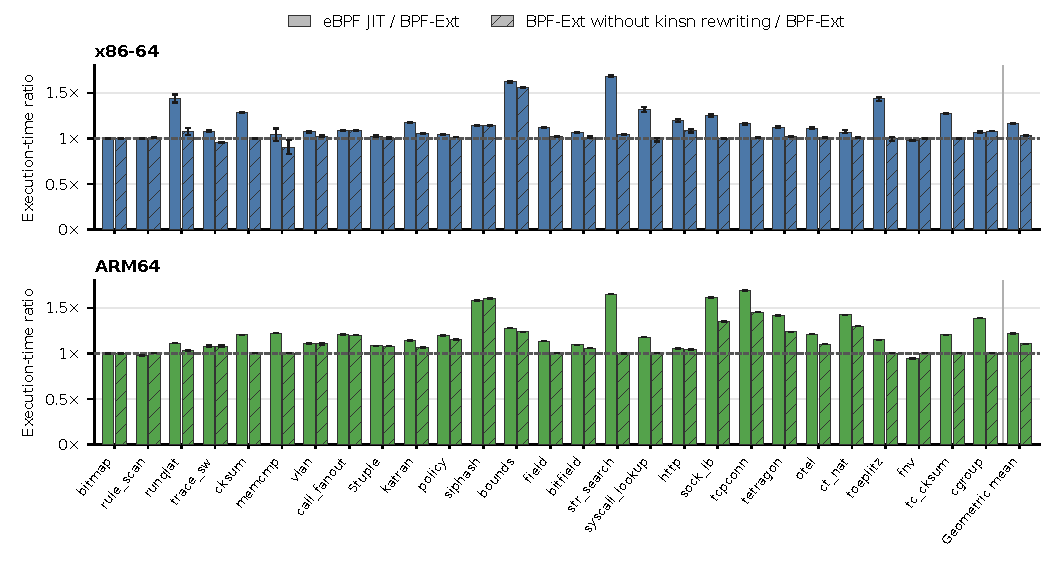
\includegraphics[width=\textwidth]{figures/sec-6-micro-performance.pdf}
\caption{Execution-time ratios for the microbenchmarks in Table~\ref{tab:microbenchmarks}. Ratios are the reference configuration's mean execution time divided by that of \tool{}. Values above 1 indicate faster execution with \tool{}. Disabling \kinsn rewriting preserves the LLVM configuration. Geometric mean summarizes the 27 ratios. Error bars show 95\% confidence intervals from paired resampling of independent instances.}
\Description{Two panels show execution-time ratios for x86-64 and ARM64 across 27 benchmarks and their geometric means. Solid bars compare eBPF JIT with BPF-Ext. Hatched bars compare BPF-Ext without kinsn rewriting with BPF-Ext. The dashed horizontal line marks equal execution time.}
\label{fig:eval-kinsn-micro}
\end{figure*}

Rewriting computations as \kinsns improves performance beyond recompilation alone. Figure~\ref{fig:eval-kinsn-micro} reports both comparisons. Relative to the eBPF JIT, \tool achieves geometric-mean speedups of 1.17$\times$ on x86-64 and 1.22$\times$ on ARM64. Relative to \tool without \kinsn rewriting, the speedups are 1.04$\times$ and 1.11$\times$, respectively. The full pipeline's gains therefore include both recompilation and \kinsn rewriting. Across the same 27 programs, the geometric mean of native code size falls by 15.1\% and 12.9\% relative to the eBPF JIT.

The benefit of \kinsn rewriting varies across programs. For example, the x86-64 string-search benchmark, \texttt{str\_search}, achieves a 1.68$\times$ speedup over the eBPF JIT but only 1.05$\times$ over \tool without \kinsn rewriting. Most of its overall gain is already present in the common compilation pipeline. ARM64 SipHash instead gains mainly from \kinsn rewriting, with corresponding speedups of 1.58$\times$ and 1.60$\times$.

A rotation ablation further identifies the benefit of this optimization in ARM64 SipHash. We disable only the rotation rule, keeping the compilation pipeline and all other rules unchanged. With rotation enabled, native rotation instructions replace 116 combinations of shifts and bitwise OR, while eight memory-access extensions remain unchanged between configurations. In a separate experiment with 12 independent instances, mean execution time falls from 121.2\,ns with rotation disabled to 77.1\,ns with rotation enabled, a 1.57$\times$ speedup and a 36.4\% reduction in execution time.

\subsection{Application Performance}
\label{subsec:corpus_application}

\begin{table*}[t]
\centering
\small
\caption{Applied optimizations in each \tool application configuration. The last column lists categories of \kinsns actually generated, using the names in Section~\ref{subsec:operations}.}
\label{tab:eval-application-configurations}
\setlength{\tabcolsep}{5pt}
\renewcommand{\arraystretch}{1.08}
\begin{tabular*}{\textwidth}{@{\extracolsep{\fill}}ll>{\raggedright\arraybackslash}p{0.48\textwidth}@{}}
\toprule
\textbf{Application} & \textbf{Configuration} & \textbf{Applied optimizations} \\
\midrule
Cilium & All optimizations & Address calculation, conditional select,\newline bulk memory access, prefetch \\
 & Without bulk memory access & Address calculation, conditional select, prefetch \\
\addlinespace
Katran & Register optimizations & Rotation, bit extraction \\
 & Register and memory optimizations & Rotation, bit extraction, big-endian load,\newline bulk memory access, prefetch \\
\bottomrule
\end{tabular*}
\end{table*}

\begin{table*}[t]
\centering
\small
\caption{Application throughput in millions of packets accepted by the sending interfaces per second (Mpps). Relative rates divide each configuration's mean by the application's eBPF JIT mean. Brackets give 95\% confidence intervals.}
\label{tab:eval-application-throughput}
\setlength{\tabcolsep}{5pt}
\renewcommand{\arraystretch}{1.08}
\begin{tabular*}{\textwidth}{@{\extracolsep{\fill}}llrc@{}}
\toprule
\textbf{Application} & \textbf{Configuration} & \textbf{Mean (Mpps)} & \textbf{Relative rate [95\% CI]} \\
\midrule
Cilium & eBPF JIT & 0.575 & 1.000 \\
 & All optimizations & 0.557 & 0.970 [0.871, 1.093] \\
 & Without bulk memory access & 0.575 & 1.000 [0.932, 1.075] \\
\addlinespace
Katran & eBPF JIT & 1.722 & 1.000 \\
 & Register optimizations & 1.710 & 0.993 [0.988, 0.998] \\
 & Register and memory optimizations & 1.721 & 0.999 [0.993, 1.005] \\
\bottomrule
\end{tabular*}
\end{table*}

\begin{table*}[t]
\centering
\small
\caption{Katran CPU costs from independent sampling. Entries give the median across three instances, with the minimum and maximum in parentheses. Estimated CPU time is divided by the increase in the virtual-IP packet counter over the same sending window. Application + callees includes kernel functions attributed to Katran through its call stacks.}
\label{tab:eval-katran-profile}
\setlength{\tabcolsep}{3pt}
\renewcommand{\arraystretch}{1.08}
\begin{tabular*}{\textwidth}{@{\extracolsep{\fill}}lcc@{}}
\toprule
\textbf{Configuration} & \textbf{Application code (ns/packet)} & \textbf{Application + callees (ns/packet)} \\
\midrule
eBPF JIT & 116.3 (114.8--118.3) & 260.4 (259.8--265.4) \\
Register optimizations & 121.5 (119.9--126.6) & 261.0 (260.6--268.5) \\
Register and memory optimizations & 121.3 (110.8--123.2) & 260.6 (259.3--269.9) \\
\bottomrule
\end{tabular*}
\end{table*}


We test whether these local optimizations improve packet-processing throughput in complete applications. Cilium~\cite{cilium} exercises a network datapath with multiple eBPF programs and tail calls, while Katran~\cite{katran} exercises XDP load balancing. Cilium uses version 1.20.0-dev on x86-64, with bidirectional IPv4 UDP traffic between two endpoints. Katran runs on ARM64, forwarding traffic from one UDP virtual IP address to one backend. Both workloads use 64-byte packets generated by two pktgen threads, each configured with 65,535 flows.

For each application, we compare the eBPF JIT with two \tool configurations. Cilium enables either all seven optimization categories in \S\ref{subsec:operations}, or the same set without bulk memory access and its associated recognition rules. Katran enables three register optimizations: rotation, conditional select, and bit extraction. A second configuration adds three memory optimizations: big-endian load, bulk memory access, and prefetch. Table~\ref{tab:eval-application-configurations} lists the categories of \kinsns actually generated under these configurations. Katran's two configurations rewrite 21 and 68 sites, respectively.

We measure application throughput after the service and datapath are ready, using 12 independent instances per configuration. Each Cilium instance warms up for 180 seconds before three 180-second measurement windows, with the Cilium agent paused during measurement. Katran uses a 30-second warmup followed by three 30-second windows. The main measurements disable BPF runtime statistics and CPU sampling. Throughput is the sum of the rates of packets accepted by the transmitting interface, as reported by the two pktgen threads. We average the three windows within each instance, then aggregate the 12 instance experiments. We compute 95\% confidence intervals for throughput ratios by jointly resampling 12 experiment batches, each containing a separate instance for every configuration.

Table~\ref{tab:eval-application-throughput} reports throughput relative to the eBPF JIT. For Cilium, enabling all optimizations yields 0.970 times the throughput obtained without bulk memory access (95\% confidence interval: [0.874, 1.083]). For Katran, adding memory optimizations to the register optimizations yields a throughput ratio of 1.006 (95\% confidence interval: [0.997, 1.015]).

To measure where CPU time is spent, we sample application code and the kernel functions it calls in separate experiments. For each Katran configuration, three fresh instances each warm up for 30 seconds before a 30-second traffic experiment with sampling. Table~\ref{tab:eval-katran-profile} reports the results. Cilium's corresponding samples appear alongside the native-compilation comparison in \S\ref{subsec:native-comparison}.

\subsection{Rewriting and First-Load Cost}
\label{subsec:preparation-cost}

\begin{table*}[t]
\centering
\small
\caption{Rewriting and first-load costs in milliseconds, using the same LLVM pipeline with and without \kinsn rewriting. Entries summarize per-program means across 27 programs. Ranges give the minimum and maximum across programs. Increments are computed per program as the cost with rewriting minus the cost without it, before summarization.}
\label{tab:eval-preparation-cost}
\setlength{\tabcolsep}{5pt}
\renewcommand{\arraystretch}{1.08}
\begin{tabular*}{\textwidth}{@{\extracolsep{\fill}}lrrrr@{}}
\toprule
 & \multicolumn{2}{c}{\textbf{x86-64}} & \multicolumn{2}{c}{\textbf{ARM64}} \\
\cmidrule(lr){2-3}\cmidrule(l){4-5}
\textbf{Measurement} & \textbf{Median} & \textbf{Range} & \textbf{Median} & \textbf{Range} \\
\midrule
Without \kinsn rewriting & 24.0 & 15.4--109.8 & 24.2 & 13.9--145.7 \\
With \kinsn rewriting & 35.6 & 24.4--138.9 & 34.2 & 23.8--155.7 \\
Per-program increment & 9.2 & 3.6--46.2 & 10.0 & 2.6--15.7 \\
\bottomrule
\end{tabular*}
\end{table*}


Local optimization adds work before program execution, so we measure the combined cost of rewriting and first loading. Using the 27 programs from \S\ref{subsec:micro_benchmark}, we compare \tool with and without \kinsn rewriting. Starting from existing bytecode, the timed stages cover userspace rewriting, reading the rewritten program, and the first object load. Object loading includes extension-target resolution and the program-loading call, which performs kernel verification and JIT compilation.

Rewriting and first loading typically take tens of milliseconds in the current implementation. Table~\ref{tab:eval-preparation-cost} summarizes the mean costs of the 27 programs. With \kinsn rewriting, the median cost is 35.6\,ms on x86-64 and 34.2\,ms on ARM64. The median per-program increase over the configuration without \kinsn rewriting is 9.2\,ms and 10.0\,ms, respectively.

The typical additional cost comes mainly from the loader's lookup of kernel implementations for \kinsns. The current loader resolves BTF information afresh on each load, taking a median of 9.1\,ms across programs on x86-64 and 9.9\,ms on ARM64. In comparison, the median increase in userspace rewriting time is 0.12\,ms and 0.14\,ms. Some x86-64 programs are recompiled after checks of rewriting conditions, adding to rewriting cost. The Katran microbenchmark's 46.2\,ms increase includes 36.6\,ms of rewriting.

Program loading is also a substantial part of preparation cost. For the string-search benchmark, which has the highest total cost, the program-loading call takes 85.8\,ms on x86-64 and 121.8\,ms on ARM64. These times include libbpf processing, kernel verification, and JIT compilation.

\subsection{Whole-Program Native Comparison}
\label{subsec:native-comparison}

\begin{table}[ht]
\centering
\small
\caption{Cilium throughput ratios, using mean rates of packets accepted by the sending interfaces. Each ratio divides whole-program native throughput by the reference throughput. Brackets give 95\% confidence intervals.}
\label{tab:eval-native-comparison}
\setlength{\tabcolsep}{3pt}
\renewcommand{\arraystretch}{1.08}
\begin{tabular}{@{}lc@{}}
\toprule
\textbf{Reference} & \textbf{Native / reference} \\
\midrule
eBPF JIT & 1.005 [0.939, 1.098] \\
All optimizations & 1.036 [0.931, 1.141] \\
Without bulk memory access & 1.005 [0.952, 1.065] \\
\bottomrule
\end{tabular}
\end{table}

\begin{table*}[t]
\centering
\small
\caption{Cilium CPU costs from independent sampling. Entries give the median across three instances, with the minimum and maximum in parentheses. Estimated CPU time is divided by packets accepted by the sending interfaces over the same sending window. Map operations include their internal callees attributed to Cilium through call stacks.}
\label{tab:eval-cilium-profile}
\setlength{\tabcolsep}{5pt}
\renewcommand{\arraystretch}{1.08}
\begin{tabular*}{\textwidth}{@{\extracolsep{\fill}}lcc@{}}
\toprule
\textbf{Configuration} & \textbf{Application code (ns/packet)} & \textbf{Map operations (ns/packet)} \\
\midrule
eBPF JIT & 208.5 (191.2--227.9) & 1,065.2 (1,027.3--2,233.9) \\
All optimizations & 198.2 (189.3--213.3) & 1,093.8 (1,050.0--1,960.8) \\
Whole-program native & 186.9 (186.1--188.6) & 1,074.6 (1,072.4--1,200.5) \\
\bottomrule
\end{tabular*}
\end{table*}


We use whole-program native compilation as a reference to compare local optimization with broader compiler optimization in an application. This experiment uses the same Cilium version and configuration as \S\ref{subsec:corpus_application}, compiles its BPF source directly to native code, and adapts the calling convention, helper calls, context access, and configuration access. Native compilation uses Clang 18.1.3 at \texttt{-O3}, targets Sapphire Rapids, and uses only general-purpose registers to meet kernel execution constraints.

This comparison trusts the entire native implementation and its integration code. The original eBPF program first passes kernel verification, after which the loader installs the native implementation before the program is attached. The verifier's acceptance of the eBPF program does not establish equivalence to its native implementation.

The native configuration uses the workload and throughput measurement procedure from \S\ref{subsec:corpus_application}, achieving a mean throughput of 0.578\,Mpps. Table~\ref{tab:eval-native-comparison} compares it directly with the eBPF JIT and both \tool configurations.

We also sample CPU time for the eBPF JIT, \tool with all seven optimization categories, and whole-program native compilation. Each configuration uses three fresh instances, with a 180-second warmup followed by one 180-second sampling window. Table~\ref{tab:eval-cilium-profile} reports the sampled costs of application code and map operations.
\section{Discussion}
\label{sec:discussion}

\tool provides a mechanism for extending local optimizations. Two research questions remain: how to build a \kinsn set useful across a broad range of programs, and how to select effective optimization combinations for a given program.

\subsection{Selecting \kinsn Operations}
\label{subsec:selecting-kinsn-operations}

An open question in constructing a \kinsn set is how to derive reusable operations from optimization opportunities in individual programs. Future work could examine this question from two perspectives: application needs and architectural capabilities. The former concerns computation and memory-access needs shared by a class of programs; the latter concerns native capabilities worth exposing through extended instructions. For example, profiling and comparing compilation results across programs could help identify candidate operations. The research question is whether these candidates can benefit a broader range of programs beyond those used to identify them.

The size of an extension set also involves a tradeoff between performance gains and maintenance costs. Adding operations enables new optimizations, but also requires reviewing kernel implementations, proving semantic equivalence, and maintaining support across architectures (Sections~\ref{sec:mechanism} and~\ref{sec:implementation}). When multiple programs and recognition rules can reuse a \kinsn, this effort supports more optimizations. Future selection methods could therefore evaluate measured gains, reuse, and maintenance costs together to determine which extensions are worth supporting over time.

\subsection{Selecting Optimizations for a Workload}
\label{subsec:selecting-workload-optimizations}

Selecting combinations of existing extensions must account for the difference between local optimization effects and whole-program performance. The number of rule matches does not capture how often each site executes or the combined performance effect of multiple rewrites. Even with a fixed extension set, research is needed on selecting rule combinations for a target program and processor, including whether selection should apply to entire rule categories or individual rewrite sites.

A challenge for automatic selection is adapting choices to different workloads while reducing manual experimentation. One direction is to combine program profiles and target-processor information in a userspace cost model that estimates the benefits of candidate rewrites, then test the selected combinations through measurement. Further questions include which inputs measurements should cover and how much workload change warrants selecting a new combination. By keeping pattern recognition in userspace, \tool allows these selection methods to develop while reusing existing \kinsn implementations.

\section{Related Work}
\label{sec:related}

We discuss related work on eBPF program optimization, operation extensions, compiler correctness, and kernel extension safety. We compare how optimizations and extensions are integrated into eBPF and how program safety and semantic preservation are established.

\noindent\textbf{eBPF program optimization.} Existing eBPF optimizations differ in where programs are transformed and how optimization results are represented. K2~\cite{xu2021synthesizing}, Merlin~\cite{mao2024merlin}, and EPSO~\cite{zhu2025epso} rewrite programs in userspace, producing bytecode in the existing eBPF instruction set. KFuse~\cite{kfuse} merges separately verified programs in the kernel, while ePass~\cite{xiang2025epass} provides a program transformation framework that cooperates with the verifier. Shahinfar et al.~\cite{shahinfar2026fun} propose post-verification optimization (PVO), in which a trusted userspace optimizer compiles verified eBPF programs into native code for kernel execution. Compared with bytecode rewriting within the existing instruction set, \tool uses \kinsns to select additional native implementations. Unlike PVO's userspace code generation, \tool checks \kinsn use and generates native code in the kernel, without trusting the userspace pattern recognizer for kernel safety.

\noindent\textbf{Extending eBPF operations.} eBPF extensions differ in how they represent and check new operations. kfuncs~\cite{kfuncs} expose kernel functions through a call interface. The verifier checks usage conditions, while function bodies remain outside bytecode analysis. hXDP~\cite{brunella2020hxdp} extends the eBPF instruction set and execution engine for FPGAs and uses hardware checks to constrain execution. Both \tool and hXDP provide additional functionality through extended instructions, but \tool targets kernel execution on CPUs and submits new operations' eBPF expansions to the existing verifier.

\noindent\textbf{Compiler correctness.} Research on verifying and synthesizing compilers for kernel domain-specific languages focuses on semantic preservation during translation. Jitk~\cite{wang2014jitk} verifies compilation paths, Jitterbug~\cite{nelson2020specification} checks BPF JIT translation steps, and JitSynth~\cite{vangeffen2020jitsynth} synthesizes correct JIT compilation fragments. Our correctness argument for \kinsns likewise requires semantic preservation: the proof concerns the correspondence between their eBPF expansions and native implementations (Section~\ref{sec:formal-verification}).

\noindent\textbf{Kernel extension safety.} Research on kernel extension safety uses mechanisms such as external proofs, language restrictions, and runtime protection. Proof-carrying code (PCC)~\cite{necula1997pcc} requires consumers to check safety proofs accompanying code. BCF~\cite{sun2025prove} improves eBPF verifier precision using external proofs checked in the kernel. KFlex~\cite{dwivedi2024fast} combines static checking of kernel interfaces with runtime protection. Rex~\cite{jia2025rex} replaces a separate bytecode verifier with a restricted subset of safe Rust, a trusted toolchain, and a runtime. MOAT~\cite{lu2024moat} and SafeBPF~\cite{soo2024safebpf} retain the verifier and add runtime memory isolation.
\section{Conclusion}
\label{sec:conclusion}

We presented \tool, which uses extended instructions to support more efficient native implementations while reusing the existing eBPF verifier. The framework keeps pattern recognition in userspace, uses eBPF implementations for safety analysis of the complete program, and executes semantically equivalent native implementations. New optimizations reuse the framework's kernel support without adding each pattern-recognition and transformation rule to the JIT. We implemented seven categories of local optimizations on x86-64 and ARM64. Relative to the stock Linux eBPF JIT, microbenchmarks achieve geometric mean speedups of 1.24$\times$ and 1.22$\times$, respectively. Throughput also improves for Cilium and Katran.


%%
%% The next two lines define the bibliography style to be used, and
%% the bibliography file.
\bibliographystyle{ACM-Reference-Format}
\bibliography{reference}

\end{document}
\endinput
%%
%% End of file `sample-sigconf-authordraft.tex'.
